% 06-language-model-exploration.tex

% Language Models Exploration
% 6.1. Introduction: Provides an overview of the language models task and its objectives.
% 6.2. Pretraining: Describes the process of pretraining Doc2Vec or using a pretrained Bert model.
% 6.3. Model Fine-tuning: Fine-tunes the last layer of the network.
% 6.4. Learning Curves: Plots learning curves and determines the optimal number of epochs.

% Section Title
\section{LANGUAGE MODEL EXPLORATION}

    % Main Content

    \subsection{Introduction}
    
        This section documents the steps taken to fine-tune a pre-trained BERT model for multi-label classification using a dataset of SSH attack sessions.
        The focus was on customizing the final classification layer and training the model on the `Set\_Fingerprint` intents. Performance metrics and visualizations are presented to evaluate the effectiveness of the model.

    \subsection{Data Preprocessing}
    
        The dataset was processed as follows:
        
        \begin{itemize}
        
            \item The `Set\_Fingerprint` column was preprocessed for multi-label encoding using the `MultiLabelBinarizer` class, enabling the representation of intents as binary vectors.
            
            \item The dataset was split into 70\% training, 20\% validation, and 10\% testing sets.
            
        \end{itemize}

    \subsection{Tokenization}
    
        Pre-trained BERT's tokenizer was used to convert text data into input IDs and attention masks. Tokenization results were saved to disk for reuse, reducing computational overhead.

    \subsection{Model Architecture}
    
        A pre-trained `bert-base-uncased` model was used, with a custom linear classification head added to predict the intents. The classifier had an input size matching BERT's hidden layer dimensions and an output size equal to the number of intents.

    \subsection{Training Process}
    
        \begin{itemize}
        
            \item The model was trained using the AdamW optimizer with a learning rate of $5 \times 10^{-5}$ and a linear scheduler.
            
            \item A `BCEWithLogitsLoss` loss function was applied for multi-label classification.
            
            \item Mixed precision training was used to enhance computational efficiency.
            
            \item Training was conducted for 4 epochs, using a gradient accumulation strategy to manage memory constraints.
            
        \end{itemize}

    \subsection{Evaluation Metrics}
    
        \begin{itemize}
        
            \item Metrics included precision, recall, F1-score, and ROC-AUC.
            
            \item ROC curves and training/validation loss curves were generated for each class.
            
        \end{itemize}

    \subsection{Results}

        \subsubsection{Training and Validation Loss \\}

            The training loss decreased steadily, indicating effective learning. However, the validation loss started increasing after epoch 2, suggesting potential overfitting. (See Figure~\ref{fig:loss}).

            \begin{figure}[h]
                \centering
                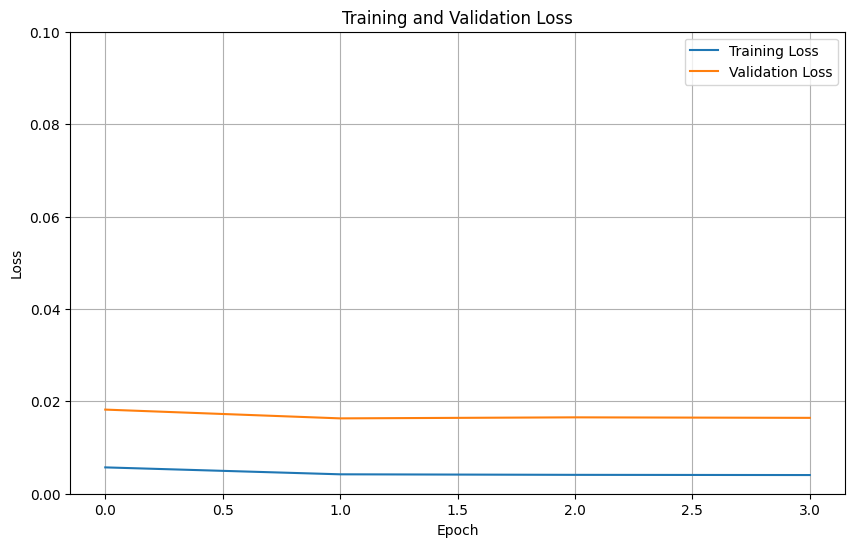
\includegraphics[width=0.7\textwidth]{../figures/plots/section4/loss_curves.png}
                \caption{Training and Validation Loss}
                \label{fig:loss}
            \end{figure}

        \subsubsection{ROC Curves \\}

            ROC curves were generated for each intent class. The area under the curve (AUC) values were as follows:
            
            \begin{itemize}
            
                \item \textbf{High AUC}: Discovery (1.00), Execution (0.98), Defense Evasion (0.97), Persistence (0.94).
                
                \item \textbf{Low AUC}: Harmless (0.77), Other (0.48), Impact (NaN due to lack of positive samples).
                
            \end{itemize}
            
            The variability in AUC values indicates that the model performs well on some intents but struggles with others. (See Figure~\ref{fig:roc}).

            \begin{figure}[h]
                \centering
                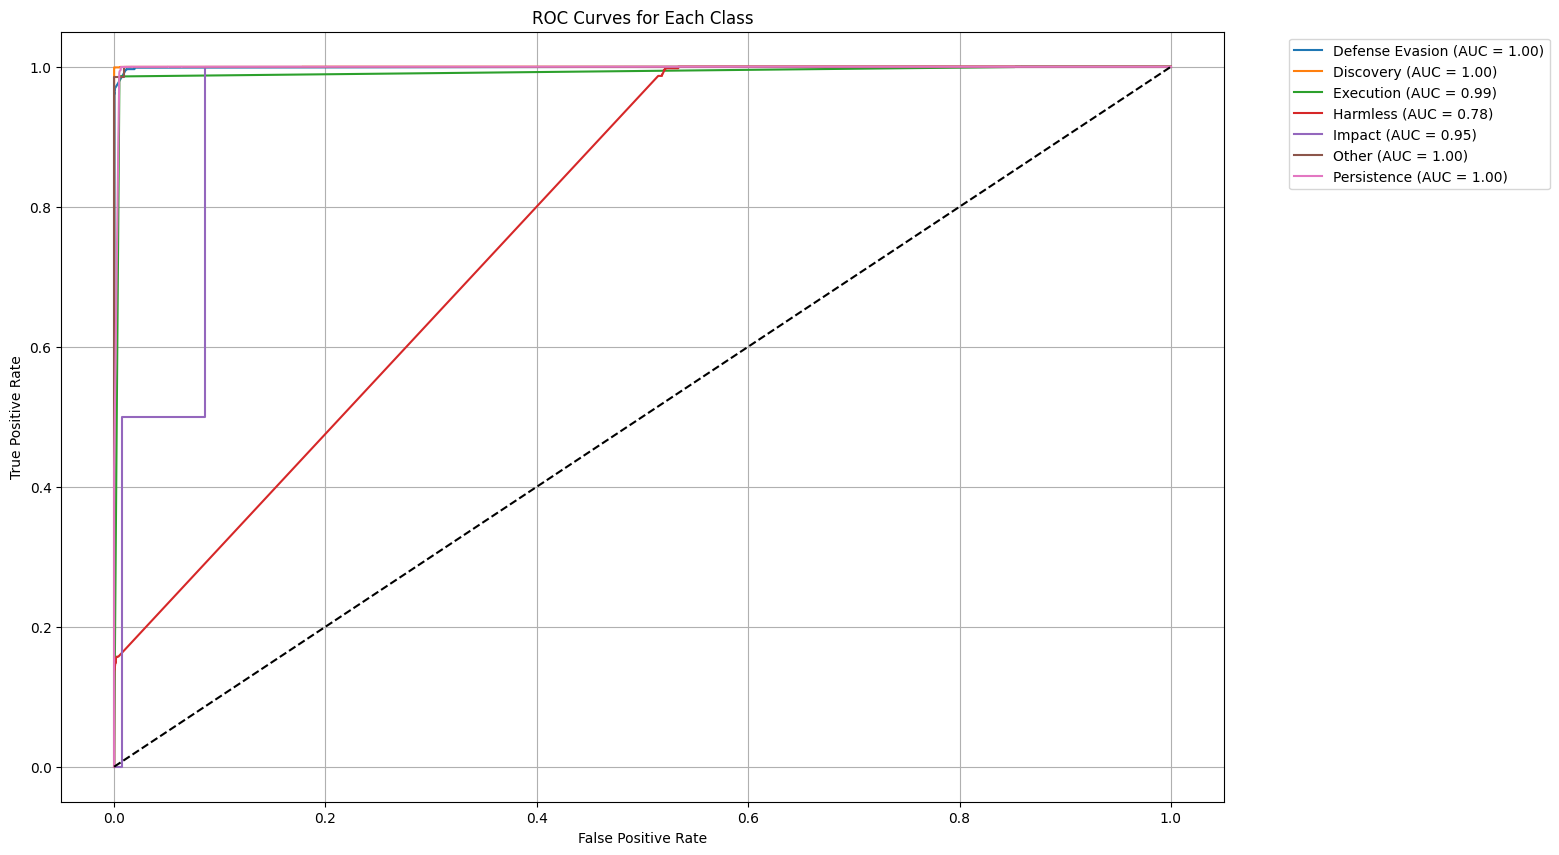
\includegraphics[width=0.9\textwidth]{../figures/plots/section4/roc_curves.png}
                \caption{ROC Curves for Each Class}
                \label{fig:roc}
            \end{figure}

        \subsubsection{Test Metrics \\}
        
            The model achieved the following metrics on the test set:
            
            \begin{itemize}
                \item Precision: 0.9974
                \item Recall: 0.9927
                \item F1-Score: 0.9937
                \item ROC-AUC: 0.9971
            \end{itemize}

    \subsection{Discussion}
    
        The results demonstrate that the fine-tuned BERT model performs well for most classes, with high AUC scores for key intents like `Discovery` and `Execution`. However, challenges remain:
        
        \begin{itemize}
        
            \item The model struggled with the `Other` class, likely due to limited or ambiguous data.
            
            \item Overfitting was observed after epoch 2, necessitating regularization techniques like dropout or early stopping in future iterations.
            
        \end{itemize}

    \subsection{Conclusion}
    
        Fine-tuning a pre-trained BERT model proved effective for multi-label classification of SSH attack intents. While the model achieved reasonable overall performance, further tuning and data argumentation could address issues with minority classes and overfitting.
